\documentclass[mathserif,serif]{beamer}
\usepackage{lmodern}
\usepackage{adjustbox}
\usepackage{multirow}
\usepackage{array}
\usepackage{csquotes}
\usepackage{color}
\usepackage{soul}
\usepackage[utf8]{inputenc}

% THEME AND LAYOUT
\usecolortheme{dove}
\beamertemplatenavigationsymbolsempty
\setbeamertemplate{footline}[frame number]
\setbeamertemplate{bibliography item}{}
\definecolor{highlightyellow}{rgb}{1,1,0.7}
\sethlcolor{highlightyellow}
\makeatletter
\newcommand\fix{%
  \let\set@color\beamerorig@set@color
  \let\reset@color\beamerorig@reset@color}
\makeatother

% TITLE PAGE
\title[TITLE] % (optional, only for long titles)
{{\bf \LARGE Auction or haggling -- \\ what should the seller choose?} \\ \large A look at the interaction between price discovery and competition in Name-Your-Own-Price auctions.}
\subtitle{}
\author[Sekamane] % (optional, for multiple authors)
{Jonas K. Sekamane}
\institute[] % (optional)
{}
\date[4 December 2014] % (optional)
{Experiments in Economics -- 4. December 2014}
\subject{PE}

% NEW COMMANDS AND TYPES
\newcolumntype{x}[1]{%
>{\raggedright\hspace{0pt}}p{#1}}%

\begin{document}
	\frame{\titlepage}
	
	\begin{frame}
		\frametitle{ }
		\vspace*{-15mm}
		\begin{figure}[plain]
			\hspace*{-11mm}
			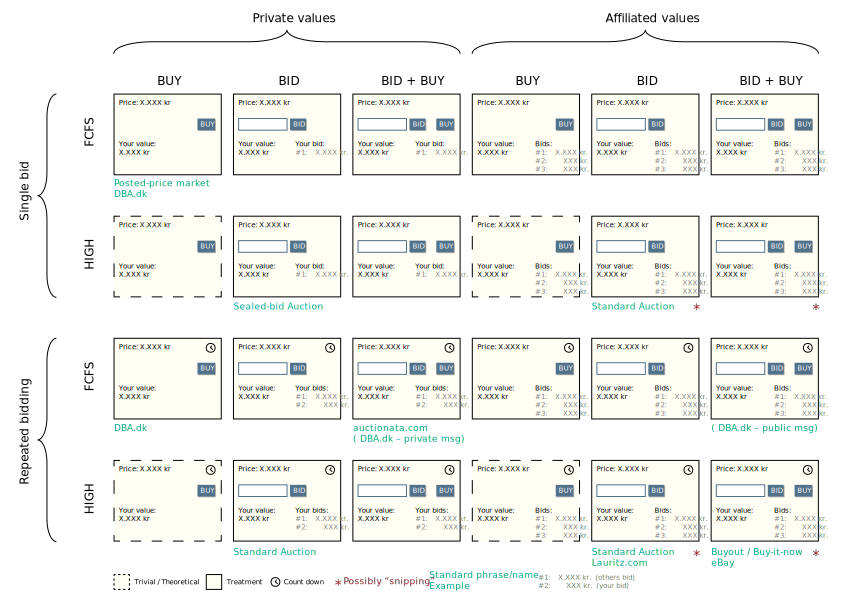
\includegraphics[width=1\paperwidth]{Figures/Overview.jpg}
		\end{figure}
	\end{frame}
	
	\begin{frame}
		\frametitle{DBA.dk -- Posted Price}
		\begin{figure}[plain]
			\hspace*{-11mm}
			\includegraphics[width=1\paperwidth]{Figures/DBA_uk.jpg}
		\end{figure}
	\end{frame}
	
	\begin{frame}
		\frametitle{Lauritz.com -- Auction}
		\begin{figure}[plain]
			\hspace*{-11mm}
			\includegraphics[width=1\paperwidth]{Figures/Lauritz.jpg}
		\end{figure}
	\end{frame}
	
	\begin{frame}
		\frametitle{auctionata.com -- NYOP}
		\begin{figure}[plain]
			\hspace*{-11mm}
			\includegraphics[width=1\paperwidth]{Figures/Auctionata.jpg}
		\end{figure}
	\end{frame}
	
	\begin{frame}
		\frametitle{auctionata.com -- NYOP}
		\begin{figure}[plain]
			\hspace*{-11mm}
			\includegraphics[width=1\paperwidth]{Figures/Auctionata_options.jpg}
		\end{figure}
	\end{frame}
	
	\begin{frame}
		\frametitle{NYOP}
		\begin{figure}[plain]
			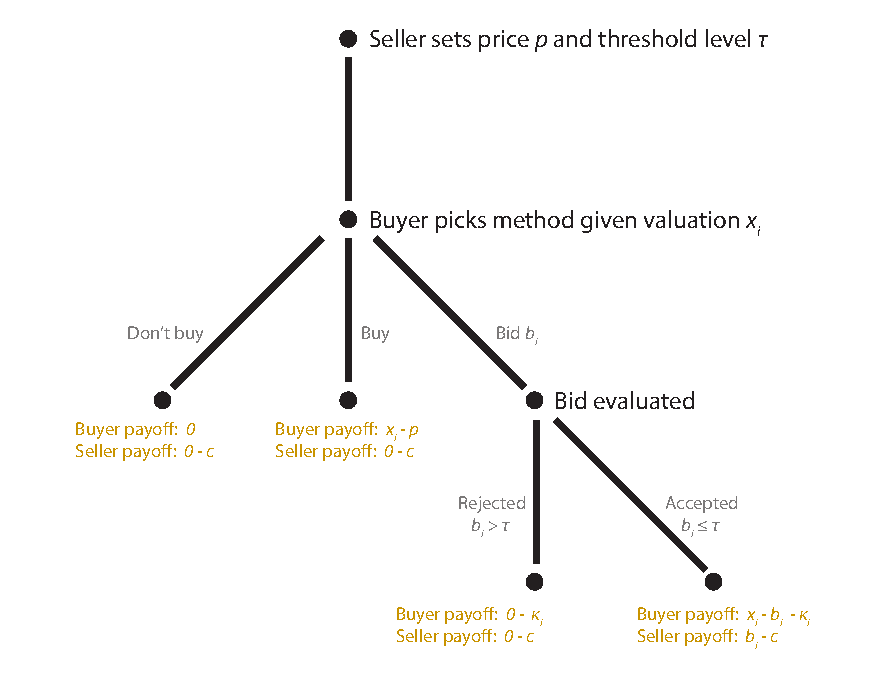
\includegraphics[width=1\textwidth]{Figures/NYOP}
		\end{figure}
	\end{frame}
	
	\begin{frame}
		\frametitle{NYOP with repeated bidding \small –– Terwiesch et. al. (2005)}
		\begin{figure}[plain]
			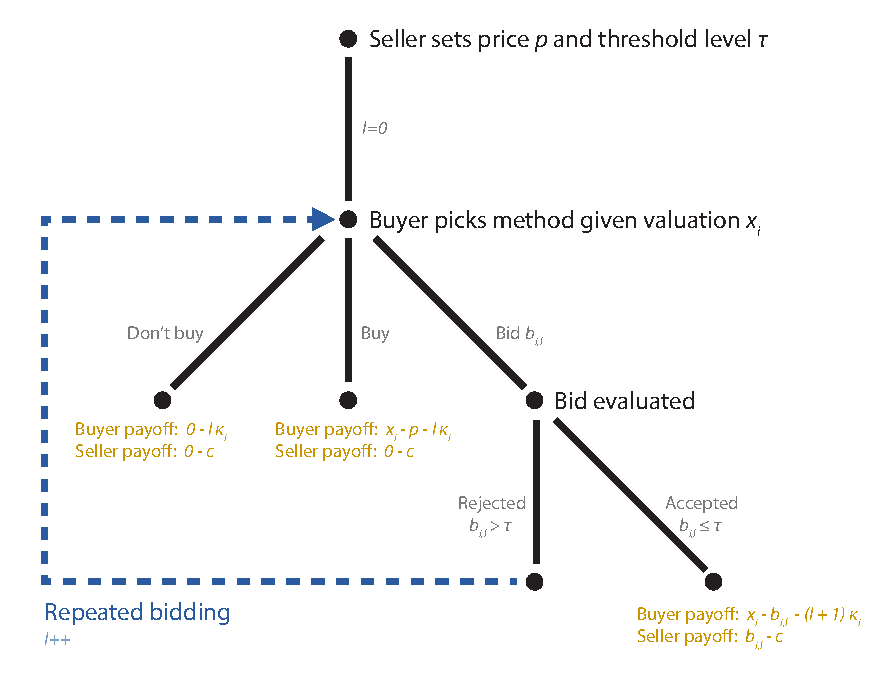
\includegraphics[width=1\textwidth]{Figures/NYOP_repeated}
		\end{figure}
	\end{frame}
	
	\begin{frame}
		\frametitle{'Haggling'}
		\begin{figure}[plain]
			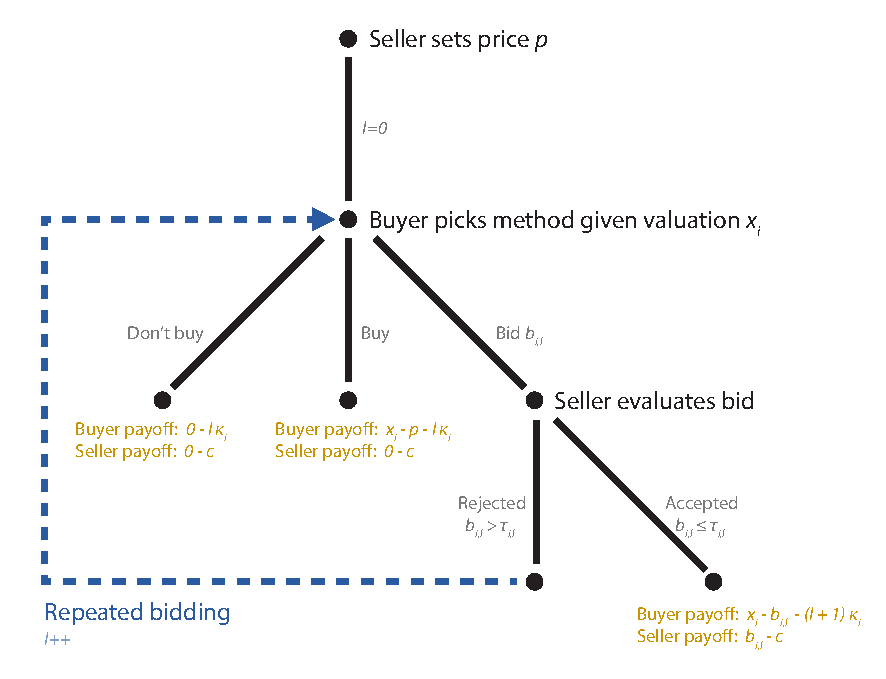
\includegraphics[width=1\textwidth]{Figures/Haggling}
		\end{figure}
	\end{frame}
	
	\begin{frame}
		\frametitle{What might happens in repeated-bidding NYOP?}

		Terwiesch et. al (2005): buyers balance between bidding too much, giving the seller additional rents -- and bidding too little, possibly enduring or wasting haggling cost.
		\begin{itemize}
			\item Bid just above: bidding repeatedly and incrementally until bid is accepted. {\bf Learning (individual channel)}.
			\item Search effort: minimise haggling costs or number of bids.
		\end{itemize}

	\end{frame}
	
	
	\begin{frame}
		\frametitle{Competition amoung buyers?}

		{\bf Auction}: Highest bid
		
		\vspace{1\baselineskip}
		
		{\bf NYOP}: {\it So far, none}.
		\vspace{1\baselineskip}
		\begin{itemize}
			\item My suggestion: 
				\begin{itemize}
					\item Scares goods / unique items.
					\item First-come-first-served (FCFS)
				\end{itemize}
		\end{itemize}

		\begin{figure}[plain]
			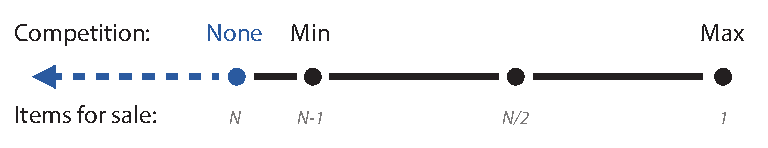
\includegraphics[width=1\textwidth]{Figures/Competition-Items}
		\end{figure}

	\end{frame}


	\begin{frame}
		\frametitle{Experiment}
		
		\begin{itemize}
			\item Participants all play the role of buyers.
			\item 5 participants in each session.
			\item Values, posted price and threshold are uniformily random:
		\end{itemize}
		\begin{figure}[plain]
			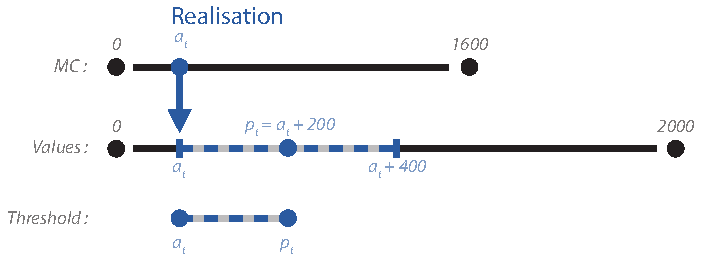
\includegraphics[width=1\textwidth]{Figures/Distribution}
		\end{figure}
		\begin{itemize}
			\item Posted price and buyer's own value is shown. (No info on distributions).
			\item Framed as scares good, e.g. {\it "One of a kind, 19th century, handpainted ..."}
		\end{itemize}
		
	\end{frame}

	\begin{frame}
		\frametitle{Treatments}
		\vspace*{-9mm}
		\begin{figure}[plain]
			\hspace*{25mm}
			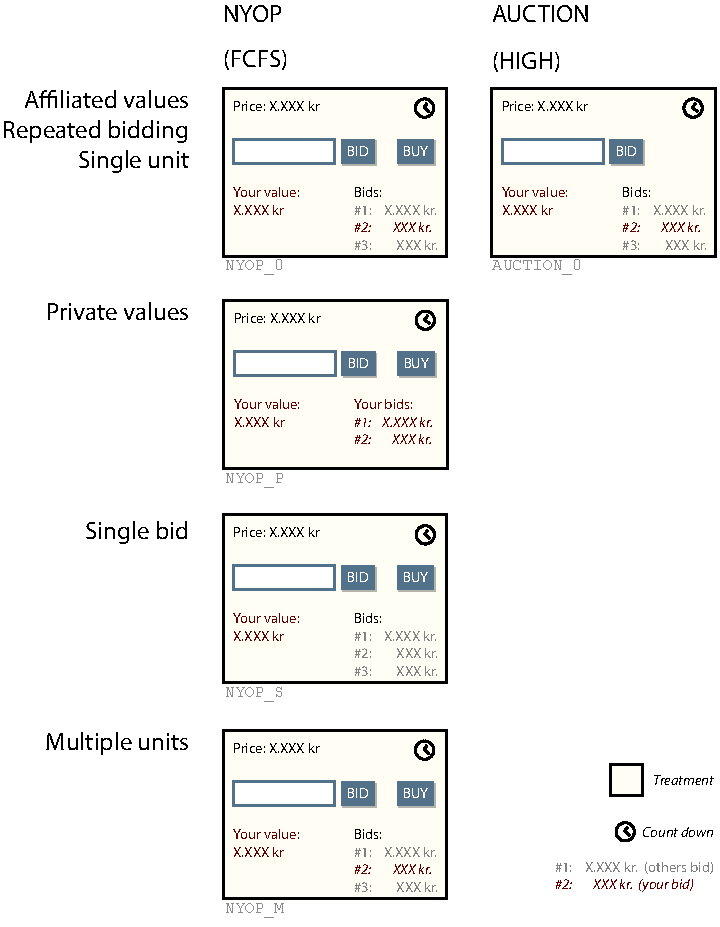
\includegraphics[height=0.98\paperheight]{Figures/Treatments}
		\end{figure}
	\end{frame}

	\begin{frame}
		\frametitle{Sessions}
			\begin{itemize}
				\item A session is 5 treatments, 8 rounds per treatment = 40 rounds.
				\item Each round last $U(60, 120)$ seconds = exp. 60 min.
				\item Randomize treatment order:
			\end{itemize}
			\[	\mbox{a}: {AUCTION_0, NYOP_0, NYOP_P, NYOP_S, NYOP_M} \]
			\[	\mbox{b}: {AUCTION_0, NYOP_M, NYOP_S, NYOP_P, NYOP_0} \]
			\[	\mbox{c}: {AUCTION_0, NYOP_P, NYOP_M, NYOP_0, NYOP_S} \]
			\[	\mbox{d}: {NYOP_M, NYOP_P, NYOP_0, NYOP_S, AUCTION_0} \]
			\[	\mbox{e}: {NYOP_S, NYOP_M, NYOP_0, NYOP_P, AUCTION_0} \]
			\begin{itemize}
				\item Initial instructions -- and again after 1st/4th treatment.
				\item End: paid baised on two randomly drawn treatments.
			\end{itemize}
	\end{frame}
	
	
	\begin{frame}
		\frametitle{}
		\vspace{2\baselineskip}
		... Thank you!
	\end{frame}

\end{document}